\documentclass[runningheads,a4paper]{llncs}
\usepackage[utf8]{inputenc}
\usepackage[T1]{fontenc}
\usepackage{csquotes}
\usepackage[english]{babel}
\usepackage[backend=bibtex,natbib,hyperref=true,maxnames=2,style=alphabetic,citestyle=alphabetic]{biblatex}
\addbibresource{seminarreport}

\usepackage{amsmath}
\usepackage{booktabs}
\usepackage{enumitem}
\usepackage{graphicx}
\usepackage{tabularx}
\usepackage{eurosym}
\usepackage[hidelinks]{hyperref}
\usepackage[capitalise]{cleveref}
\usepackage{floatrow}
\usepackage{subfig}
\usepackage[export]{adjustbox}
\usepackage{svg}

\DeclareMathOperator*{\somefunc}{somefunc}
%
\begin{document}
%
\frontmatter          % for the preliminaries
%
\pagestyle{headings}  % switches on printing of running heads
%
\mainmatter              % start of the contributions
%
\title{Self-supervised Video Prediction}
\subtitle{Lab Vision Systems - Learning Vision Systems on Graphics Cards  MA-INF 4308}
%
\titlerunning{Lab Vision Systems, Self-supervised Video Prediction }  % abbreviated title (for running head)
%
\author{Leuschner Oliver, Scheffczyk Jan}
%
\authorrunning{O. Leuschner, J. Scheffczyk }   % abbreviated author list (for running head)
\institute{Universit\"at Bonn\\
\email{s6jascef@uni-bonn.de}, Matrikelnummer: 3242317 \\
\email{s6olleus@uni-bonn.de},
Matrikelnummer: 3205025
}

\maketitle              % typeset the title of the contribution

\begin{abstract}
In this Lab we implemented and refined a convolutional neural network for supervised video prediction.  Given a set of three consecutive frames the network predicts the next three frames. The network architecture has been proposed for the lab and extends on the Video Ladder Network by utilizing additional location dependent convolutions as well as exchanging the LSTM layers to more memory efficient GRU layers. Thus we will call this model Location dependent Video Ladder Network (L-VLN). In addition we explore the possibilities for transfer learning by using the hidden states of the video prediction network for classification. This report will give a short overview of the used technologies as well as an  implementation.

\end{abstract}

\section{Introduction}
The task of video prediction consists of taking in a sequence of frames and generating succeeding frames from it. This is a challenging task, as the scene as well as it’s physical rules have to be learned by a model to make sensible predictions. Furthermore the spatial layout of a scene has to be taken into account if a scene contains static and dynamic elements. The learned internal representation of a scene can additionally be used as features for classifying the scene or the actions performed in the scene. In recent years deep neural networks have advanced many computer vision tasks including video prediction. In this work we build on previous architectures and investigate whether contemporary advancements at different parts of the architecture supplement each other.
In the video prediction task, three images are forwarded into the model which is then tasked to predict the subsequent three images. In the video classification task a full video is forwarded to the network. The hidden states of the ConvGRUs can then be used as inputs for a MLP with one hidden layer, classifying the video.


\section{Related Work}
Computer vision tasks such as object recognition have been dominated by convolutional neural networks in the recent years. Since the introduction of AlexNet \citep{krizhevsky_imagenet_2012} all new records on the ImageNet benchmark have been achieved by convolutional neural network \citep{aismartz_cnn_2019}.  These models require enormous amounts of computational power and training data which is typically only available to large corporations such as Facebook, Google or Microsoft \citep{tensorflow_how_2020}. However, these pre-trained networks can be used in numerous applications even beyond object recognition which makes state-of-the-art accuracy available to individuals and projects with much smaller data sets by utilizing transfer learning \citep{tan_survey_2018}.

The network architecture proposed for this lab utilizes the concept of transfer learning by basing their model on ResNet-18 \citep{he_deep_2015}. This network uses fewer weights in comparison to other networks in the ImageNet benchmark and is therefore suited for extensions by limited computational resources. Inspired by the Video ladder network (VLN) \citep{cricri_video_2016} lateral connections between different resolutions are used with residual layers. As ConvGru \citep{siam_convolutional_2016} reduces both computation and memory and video prediction of the few frames does not require as much long-term memory they replace the original LSTM layers. Furthermore as shown in \citep{kurkova_location_2018} location dependent convolution can help to reduce a prediction loss and video production tasks.


\begin{figure}
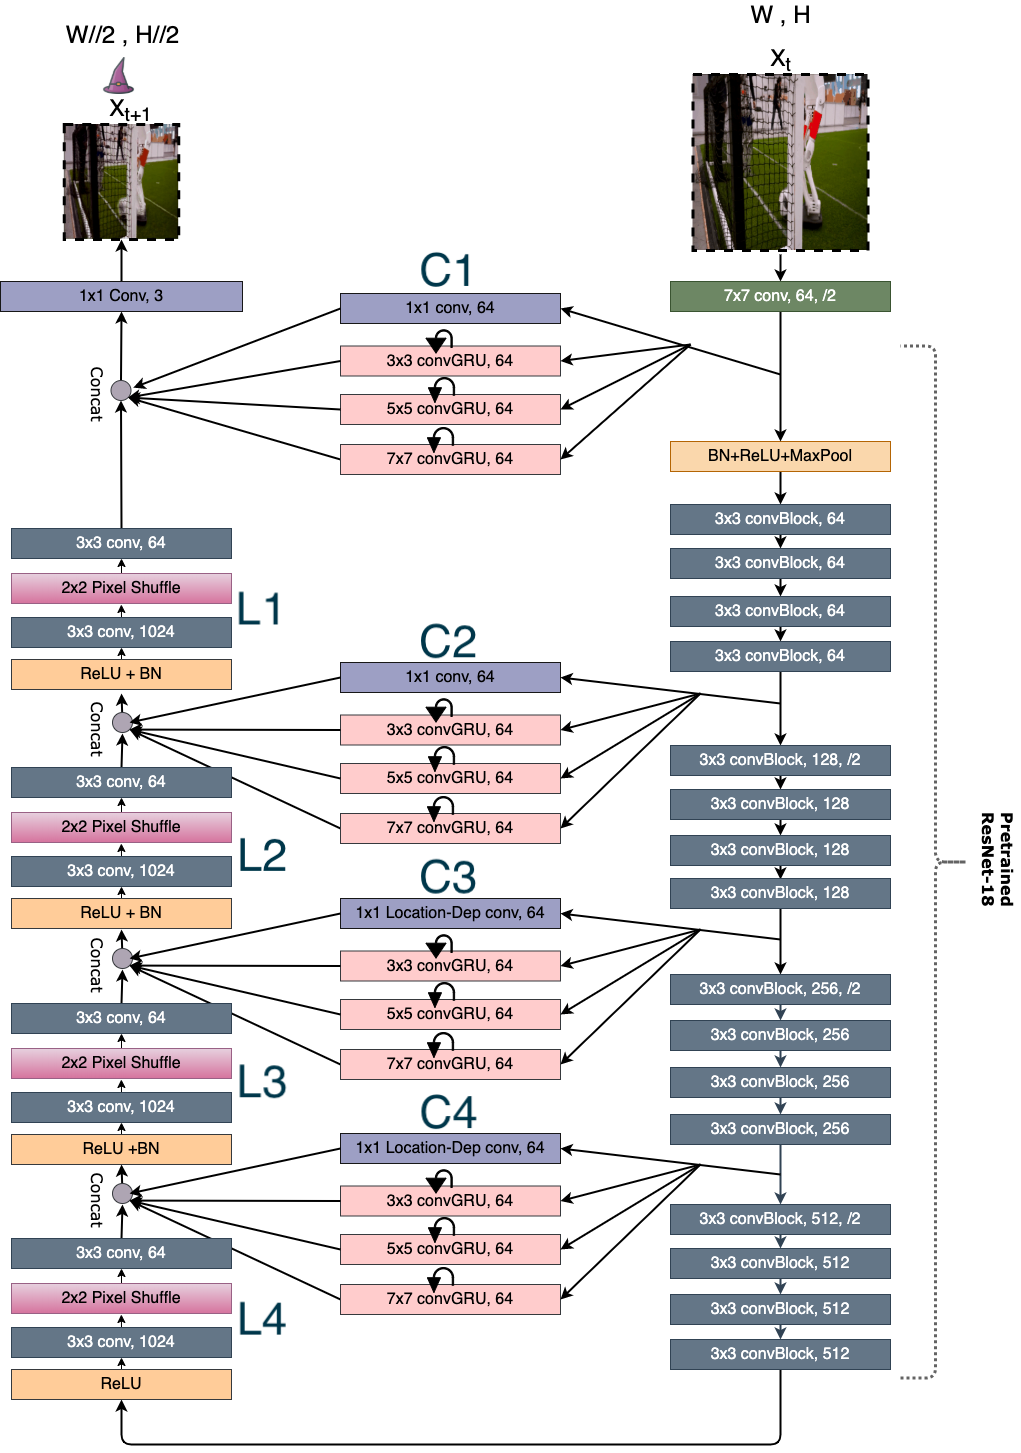
\includegraphics[width=0.45\linewidth]{res/NimbRoPred}
\caption{ L-VLN model overview as proposed for this Lab}
\label{fig:orig_arch}
\end{figure}


\clearpage
\section{Methods}
The network was implemented using pytorch and the pytorch lightning library. The project is structured into loading the data (utils/UCFLoader), defining the models (LVLN\_model, one\_frame\_model, one\_frame\_model\_full\_res) and running (main) and evaluating (sample, one\_frame\_sample) these models. This can be seen in fig. \ref{fig:project_setup}. Additionally tensorboard and weights and biases is used for monitoring the training progress.

\begin{figure}
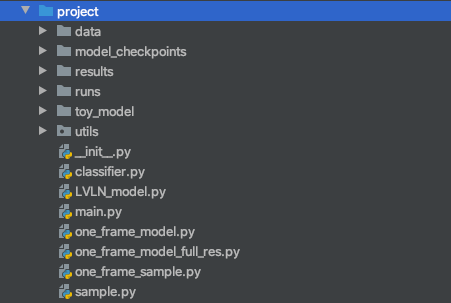
\includegraphics[width=0.45\linewidth]{res/project_setup.png}
\caption{ Setup of the project }
\label{fig:project_setup}
\end{figure}

The training and validation datasets are loaded from UCF101 videos that have been split into clips of sequences of six frames. We’ve experimented with both adapting the framerate of the video, and thus effectively increasing the time step in between each successive frame, as well as the dataset size by adapting the step size between clips, effectively reducing the size of the dataset. We settled on first training the network on 25fps and then reducing the fps after four epochs to 15 and then finally 10fps. The intuition being that the network firstly learns to correctly reproduce a scene and then focus on integrating movement by lowering the fps. Varying the step size between clips did not show any significant difference. To ensure a 0 fractional part during the integer divisions present in the four up/downsampling layers we rescaled the input to a multiple of 8 while maintaining the aspect ratio. Therefore frames are rescaled to have a height of 128 and a width of 160.  Most recurrent neural networks in pytorch take the full sequence as input, however as we generate frames that will then be used as input we augment the ConvGRU implementation accordingly. Furthermore we adapted the UCF101 loader to allow for transformations of all video frames and implemented a loader for sampling, testing and debugging that loads a single video sequence.

The first three frames are consecutively forwarded through the model. This gives the model the opportunity to learn the temporal features of the scene and differentiate between static and dynamic content. As depicted in figure \ref{fig:regular_prediction}\subref{orig_pred}, feeding these first three input frames through the network will generate the first predictive frame which will be compared to the fourth input frame. For the last two predictions the previous predictions are used as model input. The loss function is then used to measure the difference between predicted and real frames. When only using DSSIM as a loss function the network correctly learns the contour of objects in the scene. Moderate L1 and L2 loss are used to ensure correct colors. After testing SGD, Adagrad and Adam we found that Adam significantly outperforms the other options and therefore utilizes a variation AdamW \citep{kingma_adam_2014}.
\begin{figure}[htb]
\captionsetup[subfigure]{width=0.2\textwidth}
 \advance\leftskip-4cm
  \raisebox{\dimexpr-.5\height}{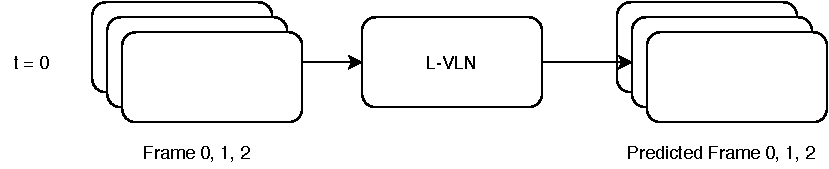
\includegraphics[scale=0.65,right]{res/original_prediction}}\ \subfloat[\label{orig_pred}]{} \\[\topskip]
  \vspace*{1.5em}
  \raisebox{\dimexpr-.5\height}{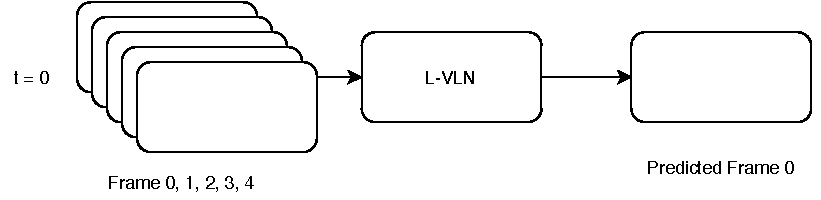
\includegraphics[scale=0.65,right]{res/mod_train}}\ \subfloat[\label{mod_train}]{}\\[\topskip]
    \vspace*{1.5em}
    \raisebox{\dimexpr-.5\height}{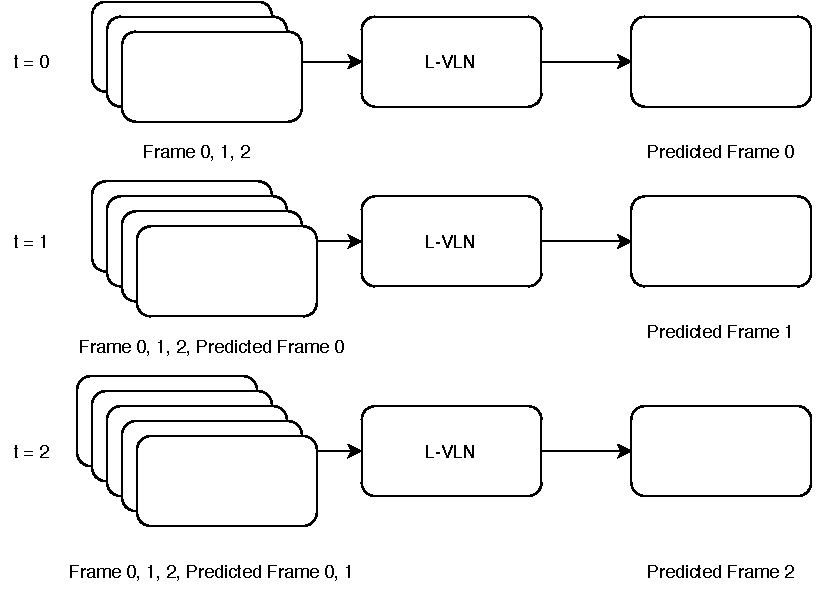
\includegraphics[scale=0.65,right]{res/mod_sample}}\ \subfloat[\label{mod_pred}]{}
  \caption{ \protect\subref{orig_pred} shows the training and predicition routine as described in the task. \protect\subref{mod_train} shows our modified training and \protect\subref{mod_pred} our modified prediction routine. }
  \label{fig:regular_prediction}
\end{figure}
The architecture can be divided into three major parts. A ResNet18 component with frozen weights, encoding the input, where the output after each block of convolutions is saved. The decoding part that consists of four blocks, L1 to L4 fig. \ref{fig:orig_arch}, upsampling the frames again. These blocks consist of firstly a batch norm and ReLU activation layer, followed by a convolutional layer, a pixel shuffle layer tasked with upsampling the image and another convolutional layer. Lastly we’ve implemented four blocks, C1 to C4 fig. \ref{fig:orig_arch}, working as latent connections between the encoding and decoding parts of the network. These blocks contain 3 ConvGRUs that learn the temporal features of the scene and one convolution layer. In the deeper two blocks the convolution is exchanged with a location dependent Convolution \cite{kurkova_location_2018} in order to encode additional location dependent features. We trained the network on a Nvidia 1080Ti GPU with a batch size of 16. One batch entry consists of a sequence of 6 frames. The training progress is continually saved to the disk and can therefore be stopped and restarted at any time.

\section{Implementation Details}
To confirm, check and debug the L-VLN we first implemented a simplified model. As a simplified dataset we use the horizontal translation of a circle to check if the temporal ConvGRU modules correctly capture and predict the movement. We augment this sample by shifting and mirroring the sequence to get a training set of 5 samples. Both models succeed at learning the motion, as can be seen in figure \ref{fig:moving_ball}.
\begin{figure}[htb]
\captionsetup[subfigure]{width=0.2\textwidth}
 \advance\leftskip-4cm
  \raisebox{\dimexpr-.5\height}{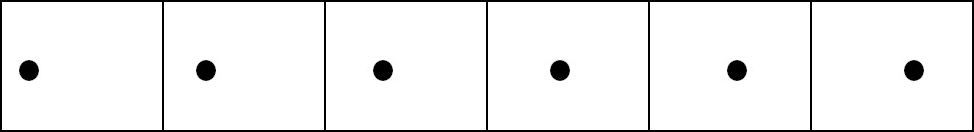
\includegraphics[scale=0.25,right]{res/moving_dot_sample_in.png}}\ \subfloat[\label{label-1}]{} \\[\topskip]
  \raisebox{\dimexpr-.5\height}{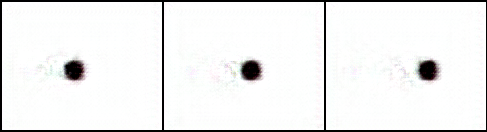
\includegraphics[scale=0.25,right]{res/moving_dot_sample_crop.png}}\ \subfloat[\label{label-2}]{}
  \caption{ \protect\subref{label-1} depicts the three input frames and the teacher images used to compare the predictions in \protect\subref{label-2} against. This example took about 500 training steps on the augmented circle dataset.}
  \label{fig:moving_ball}
\end{figure}

\begin{figure}[htb]
\captionsetup[subfigure]{width=0.2\textwidth}
 \advance\leftskip-4cm
  \raisebox{\dimexpr-.5\height}{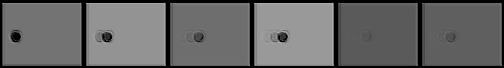
\includegraphics[scale=0.45,right]{res/gru_filter_before_training.png}}\ \subfloat[\label{label-1}]{} \\[\topskip]
  \raisebox{\dimexpr-.5\height}{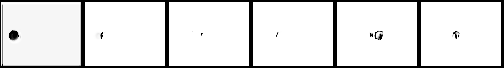
\includegraphics[scale=0.45,right]{res/gru_filter_after_training.png}}\ \subfloat[\label{label-2}]{}
  \caption{ A single filter of a ConvGRU throughout the training process, before and after training the model }
  \label{fig:gru_filter}
\end{figure}


 Further we confirm that the hidden state captures and retains salient information throughout the time series, see Figure \ref{fig:gru_filter}.
  After verifying that all components work as expected we then test whether the L-VLN can predict movement on subsets of length 5 (fig.\ref{fig:set5}), 20 (fig. \ref{fig:set20}), 40 (fig. \ref{fig:set40}) of the UCF101 dataset.

   These experiments showed us that we require a training loss of less than 0.1 to achieve results as above. Finally we proceeded to train on 25\% of the full dataset for 140 epochs (300.000 training steps) which took us 6 days\footnote{And roughly 18\euro \ in electricity cost}  on our hardware, fig. \ref{fig:predicition_comparison} \subref{threeFrameOut}. More samples can be found in the appendix \ref{fig:random_6_comb}. During training the pre-trained weights from the ResNet component where not updated.


Unfortunately the L-VLN model fails to predict movement within the images on larger datasets and instead only blurs the regions containing movement. The loss curve does not indicate that results will significantly improve within a reasonable timeframe since the loss hovers far above 0.8.

\begin{figure}[htb]
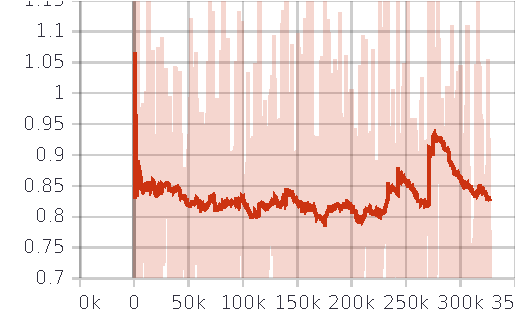
\includegraphics[scale=0.75]{res/train_loss_three_frame.pdf}
\caption{ Training loss of the full L-VLN model over a 300k training step period. }
\end{figure}

To avoid artifacts from values outside the defined 0, 1 range for rgb values we clip all images to this range before displaying, see fig.\ref{fig:artifact}.
By ensuring that the coefficients of the three different losses sum to one their ratio can be changed without affecting the learning rate.

\begin{figure}[H]
\captionsetup[subfigure]{width=0.2\textwidth}
 \advance\leftskip-4cm
  \raisebox{\dimexpr-.5\height}{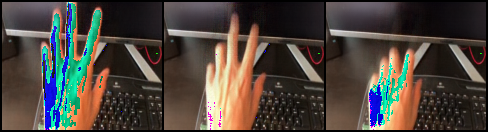
\includegraphics[scale=0.25,right]{res/with_artifacts.png}}\ \subfloat[\label{label-1}]{} \\[\topskip]
  \raisebox{\dimexpr-.5\height}{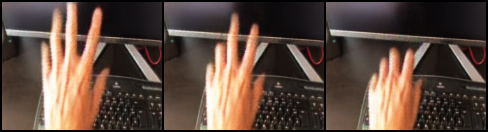
\includegraphics[scale=0.25,right]{res/no_artifacts.png}}\ \subfloat[\label{label-2}]{}
  \caption{ shows result with \protect\subref{label-2} and without \protect\subref{label-1} clipping. }
  \label{fig:artifact}
\end{figure}


\subsection{Simplifications}
The previous experiments suggest that either the problem complexity is too high for the proposed L-VLN model, or we lack the computational resources to adequately train the 31 million parameters. We therefore propose to reduce the problem complexity by predicting only a single frame at a time, given a sequence of varying length. For training we use seeding sequences of 5 frames to predict the sixth frame. However, the model works independent of the length of the seeding sequence. This allows us to append predictions to the seeding frames in order to predict a second and finally third frame. Therefore we can predict three frames similarly to the previous approach. Further to reduce the computational requirements we reduced the input size further, down to 64 by 96 pixels.
The proposed L-VLN model returns a predicted image of half the resolution of the input image. In order to compute the loss the output has to be upsampled or the ground truth frames have to be downsampled. As we’re already working with fairly small images downsampling them further masks small motion in the process. Therefore we chose to upsample instead before computing the loss. We added a pixel shuffle \citep{shi_real-time_2016} before the output that is responsible for the upsampling. While this works well for images in the training set it results in a notable grid pattern on novel data. To ensure that these artifacts are not solely based on the added pixel shuffle we also tried a bilinear and nearest neighbour upsampling, see fig. \ref{fig:artifacts}, which resulted in similar but not as severe grid structures. Otherwise this approach manages to predict motion, even on unseen data, unlike the previous attempt fig. \ref{fig:predicition_comparison} \subref{oneFrameOut}.
\begin{figure}[H]
\captionsetup[subfigure]{width=0.2\textwidth}
 \advance\leftskip-4cm
  \raisebox{\dimexpr-.5\height}{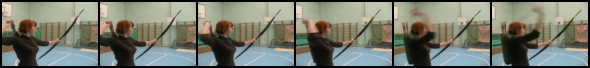
\includegraphics[scale=0.45,right]{res/one_frame_predict_3days_in.png}}\ \subfloat[\label{label-1}]{} \\[\topskip]
  \raisebox{\dimexpr-.5\height}{\includegraphics[scale=0.272,right]{res/threeFrame_6days_out.png}}\ \subfloat[\label{threeFrameOut}]{} \\[\topskip]
  \raisebox{\dimexpr-.5\height}{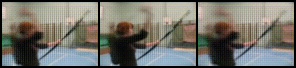
\includegraphics[scale=0.45,right]{res/one_frame_predict_3days_out.png}}\ \subfloat[\label{oneFrameOut}]{} \\[\topskip]
  \raisebox{\dimexpr-.5\height}{\includegraphics[scale=0.45,right]{res/one_frame_predict_fullRes_out.png}}\ \subfloat[\label{fullResOut}]{}

  \caption{ \protect\subref{threeFrameOut} shows results after training for 300.000 training steps using the original approach, \protect\subref{oneFrameOut} and \protect\subref{fullResOut} show the results after training with the single frame approach and the modified architecture respectively. }
  \label{fig:predicition_comparison}
\end{figure}

\subsection{Full resolution improvements}
The grid structures appear to be caused by the upsampling. Therefore we tried to adjust the model, fig. \ref{fig:modified_arch}, such that it inherently predicts frames of the same resolution. This also requires to reduce the filter, size as the ConvGRU modules are now working on full resolution images. The training uses the same one frame prediction approach as described in section 4.1. While this does address and solve the grid structures we suspect that effective increase of resolution inside the model would again require more computational resources than we have available. See figure \ref{fig:predicition_comparison} \subref{fullResOut}.
\begin{figure}[!tbp]
  \centering
  \begin{minipage}[b]{0.2\textwidth}
    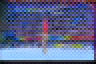
\includegraphics[width=\textwidth]{res/artifact_nearest.png}
 %   \caption{Flower one.}
  \end{minipage}
  \hfill
  \begin{minipage}[b]{0.2\textwidth}
    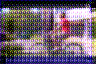
\includegraphics[width=\textwidth]{res/artifacts_shuffle.png}
%    \caption{Flower two.}
  \end{minipage}
  \hfill
  \begin{minipage}[b]{0.55\textwidth}
    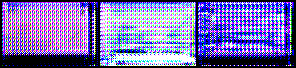
\includegraphics[width=\textwidth]{res/one_frame_predict_3days_art_out.png}
%    \caption{Flower two.}
  \end{minipage}
  
  \caption{ Artifacts using nearest neighbor upsampling and pixel shuffle. Occurence and intensity increase as training progresses. Therefore early stopping was used for all other one frame samples in this section. }
  \label{fig:artifacts}
\end{figure}


\section{Classification}
For the video classification task we use our pretrained video prediction model from the previous task, fig. \ref{fig:regular_prediction}\subref{orig_pred}, as base component. The frames of a video get propagated through the network but we disregard the output. After all frames are forwarded the states of the ConvGRUs are extracted as features for the classification.
They are then used as input for a fully connected neural network with one hidden layer and one output layer. Since concatenating all hidden states of all ConvGRUs results in over 1 billion parameters it is computationally not feasible to do so. We then experimented with different strategies for choosing which filters to use as input to the fully connected layers. We reasoned that the hidden states in the deepest latent connection, which are part of the C4 block, should contain the most compressed representation of the sequence. We compared this to subsampling all hidden states. Finally we combined both approaches by sampling all of the deepest filters and additionally taking a subsample of the other hidden states. In addition we tried Batch Normalization and Dropout for regularization, but removed Dropout since it decreased accuracy. As a loss function we use Cross entropy loss and optimize the parameters with Adam. We test the accuracy on the validation set and reach an accuracy of up to 59\% on the full validation set. The learning progress can be seen in fig \ref{fig:class_comp}.

\begin{figure}
\includegraphics[width=0.85\linewidth]{res/class_comp}
\caption{ Comparison of validation accuracy between different normalization methods (BN batch normalization, DO dropout 0.3). Validation has been performed every 0.03 epochs on 5\% of the validation set. }
\label{fig:class_comp}
\end{figure}
 

\section{Conclusion}
We have shown that the L-VLN architecture is, in principle, able to predict motion in video frames as shown with both a moving circle and small training sets. We explored multiple simplifications to make training on the full dataset feasible. This allowed us to achieve rudimentary motion prediction with only 6 days of training on a single GPU. Then we tried to adopt the model to address the grid artifacts and possibly improve sharpness. For this we proposed a slight alteration of the L-VLN model. Finally we show that the hidden states of the ConvGRU model can be used for action classification.

\printbibliography
\section{Appendix}

\begin{figure}[htb]
\captionsetup[subfigure]{width=0.2\textwidth}
 \advance\leftskip-4cm
  \raisebox{\dimexpr-.5\height}{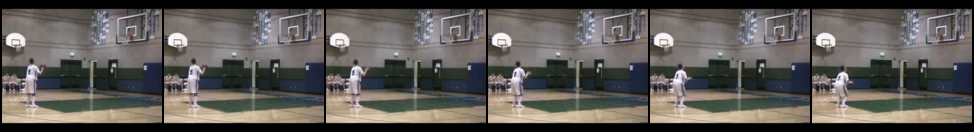
\includegraphics[scale=0.25,right]{res/set_5_in.png}}\ \subfloat[\label{label-1}]{} \\[\topskip]
  \raisebox{\dimexpr-.5\height}{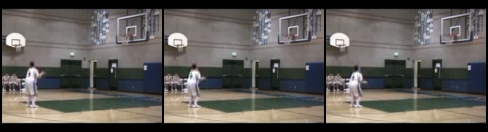
\includegraphics[scale=0.25,right]{res/set_5.png}}\ \subfloat[\label{label-2}]{}
  \caption{ \protect\subref{label-1} depicts the three input frames and the teacher images used to compare the predictions in \protect\subref{label-2} against. This example was trained on a trainingset of size 5.}
  \label{fig:set5}
\end{figure}
\begin{figure}[htb]
\captionsetup[subfigure]{width=0.2\textwidth}
 \advance\leftskip-4cm
  \raisebox{\dimexpr-.5\height}{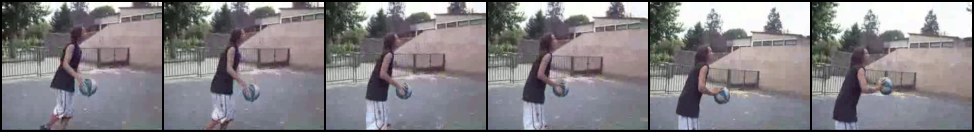
\includegraphics[scale=0.25,right]{res/set_20_2_in.png}}\ \subfloat[\label{label-1}]{} \\[\topskip]
  \raisebox{\dimexpr-.5\height}{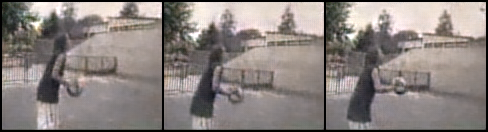
\includegraphics[scale=0.25,right]{res/set_20_2.png}}\ \subfloat[\label{label-2}]{}
  \caption{ \protect\subref{label-1} depicts the three input frames and the teacher images used to compare the predictions in \protect\subref{label-2} against. This example was trained on a trainingset of size 20.}
  \label{fig:set20}
\end{figure}
\begin{figure}[htb]
\captionsetup[subfigure]{width=0.2\textwidth}
 \advance\leftskip-4cm
  \raisebox{\dimexpr-.5\height}{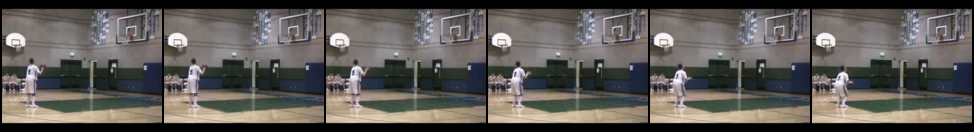
\includegraphics[scale=0.25,right]{res/set_5_in.png}}\ \subfloat[\label{label-1}]{} \\[\topskip]
  \raisebox{\dimexpr-.5\height}{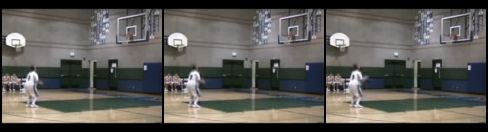
\includegraphics[scale=0.25,right]{res/set_40_3.png}}\ \subfloat[\label{label-2}]{}
  \caption{ \protect\subref{label-1} depicts the three input frames and the teacher images used to compare the predictions in \protect\subref{label-2} against.This example was trained on a trainingset of size 40.}
  \label{fig:set40}
\end{figure}

\begin{figure}[htb]
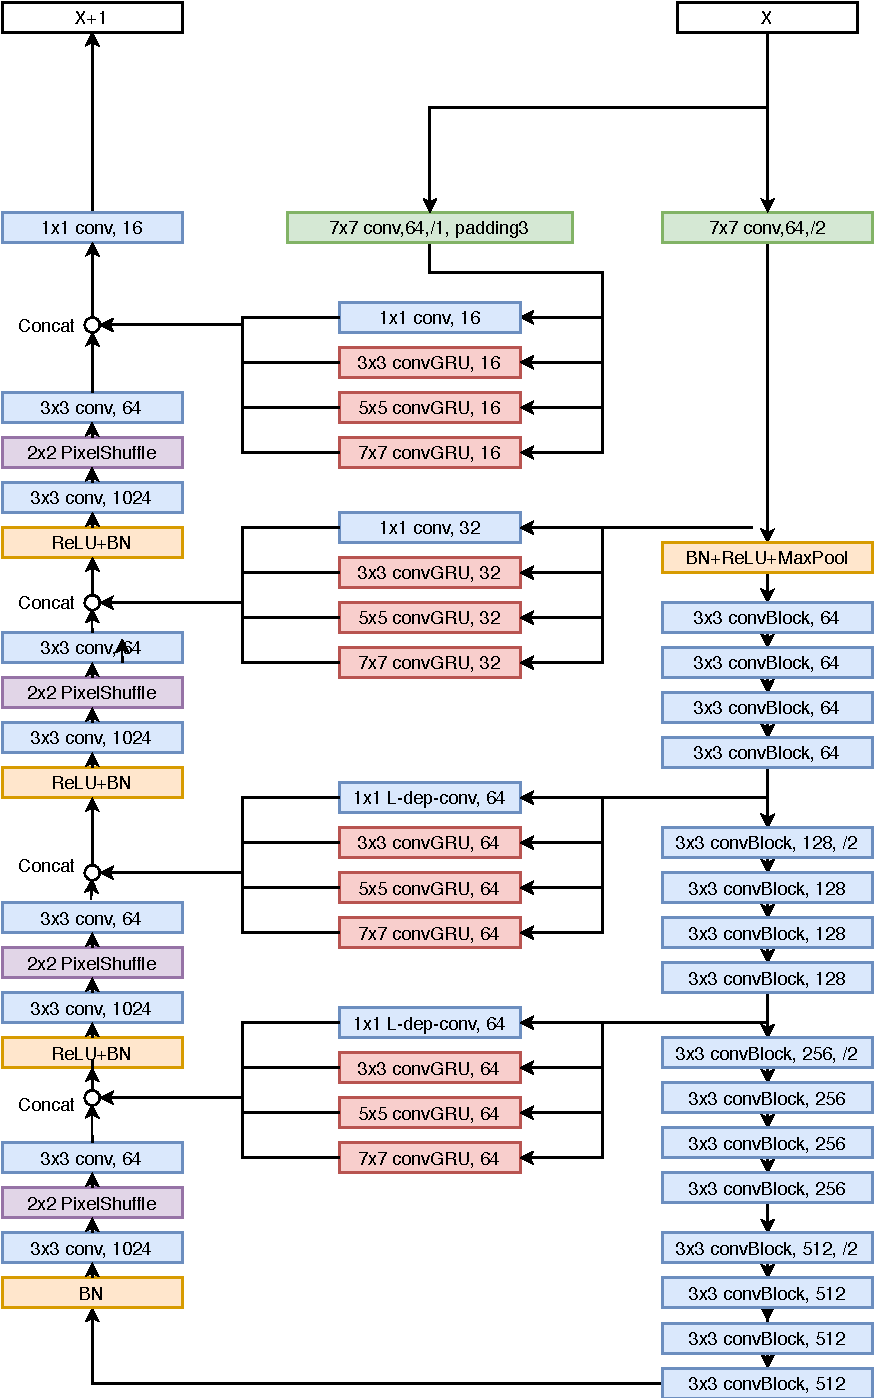
\includegraphics[scale=0.75]{res/experiment.pdf}
\caption{ L-VLN architecture modified for improved full resolution prediction and reduced memory consumption }
\label{fig:modified_arch}
\end{figure}


\begin{figure}[htb]
\includegraphics[width=\textwidth]{res/random_6_comb.png}
\caption{ Samples generated by the one frame approach }
\label{fig:random_6_comb}
\end{figure}



\end{document}
